\documentclass[a4paper]{article}
% Pacotes necessários
\usepackage[portuguese]{babel}
\usepackage[backend=biber, style=apa, citestyle=apa, language=portuguese]{biblatex}
\usepackage{csquotes}
\addbibresource{Recursos/referencias.bib}

\usepackage{amsmath}
\usepackage{graphicx}
\usepackage{subcaption}
\usepackage{setspace}
\usepackage{siunitx} % Required for alignment
\sisetup{
  round-mode          = places, % Rounds numbers
  round-precision     = 2, % to 2 places
}
\usepackage{enumerate}
\usepackage{enumitem}
\usepackage{amsmath}
\usepackage{karnaugh-map}
\usepackage[section]{placeins}
\usepackage{geometry}
\usepackage{amssymb}
\usepackage{titling}
\usepackage[T1]{fontenc}
\usepackage{float}
\usepackage[hidelinks]{hyperref}
\usepackage{xcolor}
\usepackage{indentfirst}
\usepackage{array}
\usepackage{soul}
\usepackage{afterpage}
\newcolumntype{P}[1]{>{\centering\arraybackslash}p{#1}}
\onehalfspacing


% Comando para criar uma página vazia
\newcommand\myemptypage{
    \null
    \thispagestyle{empty}
    \addtocounter{page}{-1}
    \newpage
}

% Página de título principal
\newcommand{\firsttitlepage}{
    \begin{titlepage}
        \centering
        \vspace*{1cm}
        
        % Logos superior
        \begin{figure}[h!]
            \centering
            
\includegraphics[width=6cm]{Recursos/LOGO_IPB} % Substitua pelo caminho da imagem
            \vspace{0.5cm}
        \end{figure}

        % Informações da instituição
        \large\textbf{INSTITUTO POLITÉCNICO DE BEJA} \\
        \large\textbf{Escola Superior de Tecnologia e Gestão} \\
        \large\textbf{Licenciatura em Engenharia Informática} \\
        \large\textbf{Sistemas de Informação} \\
        
        \vspace{2cm}
        
        % Título do projeto
        {\Huge \textbf{Trabalho de Grupo 1}} \\
        
        \vspace{1.5cm}
        
        % Autores
        \large Martinho José Novo Caeiro - 23917 \\
        \large Paulo António Tavares Abade - 23919 \\
        
        \vfill
        
        % Logo inferior
        \begin{figure}[h!]
            \centering
            
\includegraphics[width=6cm]{Recursos/IPBejaESTIG.jpg} % Substitua pelo caminho da imagem
        \end{figure}
        
        \vspace{1cm}
        
        % Local e data
        {\large Beja, novembro de 2024}
    \end{titlepage}
}

\newcommand{\secondtitlepage}{
    \begin{titlepage}
        \centering
        \vspace*{1cm}
        
        % Informações da instituição
        \large\textbf{INSTITUTO POLITÉCNICO DE BEJA} \\
        \large\textbf{Escola Superior de Tecnologia e Gestão} \\
        \large\textbf{Licenciatura em Engenharia Informática} \\
        \large\textbf{Sistemas de Informação} \\
        
        \vspace{2cm}
        
        % Título do projeto
        {\Huge \textbf{Trabalho de Grupo 1}} \\
        
        \vspace{1.5cm}
        
        % Autores
        \large Martinho José Novo Caeiro - 23917 \\
        \large Paulo António Tavares Abade - 23919 \\

        \vspace{2cm}

        % Orientador
        \large Orientador: Professora Isabel Sofia Brito \\
        
        \vfill
        
        % Local e data
        {\large Beja, novembro de 2024}
    \end{titlepage}
}

\begin{document}


\pagenumbering{gobble} % Oculta numeração da página

% Primeira página de título
\firsttitlepage

\secondtitlepage


% Abstract
\section*{\LARGE\textbf{\textit{Resumo}}}

Este trabalho consiste na análise de informações relativas a carros entre os anos 1970 e 1982, compreender a sua evolução 
e como a Crise do Petróleo influenciou a produção e desenvolvimento dos carros, 
alterando o motor e por consequência a sua aceleração, eficiência e consumo. 
Para tal, foi utilizada uma base de dados com 393 entradas, com 9 atributos iniciais, 
sendo estes: Milha por Galão, Cilindros, Cilindrada, Cavalagem, Peso, Aceleração, Ano de Fabrico, 
País de Origem e o Nome Completo do Carro. 
Ainda foi utilizada outra base de dados que indica o preço médio de combustível por ano, entre 1970 e 1982, 
nos Estados Unidos da América. O desenvolvimento necessitou da utilização do Excel, PowerQuery e SQL Server Management, para a criação de uma Data Warehouse. 
A nossa teoria é que a Crise do Petróleo influenciou a produção e o desenvolvimento dos carros entre os anos 1970 e 1980, alterando o motor e por consequência a sua aceleração, eficiência e consumo.




\vspace{1cm}
% Keywords
\textbf{Keywords:} excel, powerquery, sql, data warehouse, etl, olap, eficiência, análise de dados, crise do petróleo, carros,
cavalagem, aceleração, eficiência, consumo, milhas por galão, cilindros, cilindrada, preço da gasolina.
\newpage
%--------------------------------------------------------------------------------------------------------------------------------------

\section*{\LARGE\textbf{\textit{Abstract}}}

This work consists of analyzing information relating to cars between the years 1970 and 1982, understanding their evolution 
and how the Oil Crisis influenced the production and development of cars, 
changing the engine and consequently its acceleration, efficiency and consumption. 
To this end, a database with 393 entries was used, with 9 initial attributes, 
these being: Mile per Gallon, Cylinders, Displacement, Horsepower, Weight, Acceleration, Year of Manufacture, 
Country of Origin and Full Name of the Car. 
Another database was used that indicates the average price of fuel per year, between 1970 and 1982, 
in the United States of America. The development required the use of Excel, PowerQuery and SQL Server Management, to create a Data Warehouse. 
Our theory is that the Oil Crisis influenced the production and development of cars between the 1970s and 1980s, changing the engine and consequently its acceleration, efficiency and consumption.




\vspace{1cm}
% Keywords
\textbf{Keywords:} excel, powerquery, sql, data warehouse, etl, olap, efficiency, data analysis, oil crisis, cars,
horsepower, acceleration, efficiency, consumption, miles per gallon, cylinders, displacement, gasoline price.
\renewcommand{\contentsname}{Índice}       % Título do sumário
\renewcommand{\listfigurename}{Índice de Figuras} % Título da lista de figuras

% Início do conteúdo do relatório
\newpage
\doublespacing
\tableofcontents
\listoffigures
\doublespacing

\newpage
\pagenumbering{arabic}

\section{Introdução}\label{intro}
Neste trabalho irá ser abordado como a Crise do Petróleo influenciou a produção e desenvolvimento
dos carros entre os anos 1970 e 1980, alterando o motor e por consequência a sua aceleração, eficiência e consumo.

Para analisar esta situação foi utilizada uma base de dados com 393 entradas, com 9 atributos iniciais, sendo estes:
 Milha por Galão, Cilindros, Cilindrada, Cavalagem, Peso, Aceleração, Ano de Fabrico, País de Origem e o Nome Completo do Carro.

Ainda foi utilizada outra base de dados que indica o preço médio de combustível por ano, entre 1970 e 1982, 
nos Estados Unidos da América.

Por fim, a nossa teoria é que a Crise do Petróleo influenciou a produção e 
desenvolvimento dos carros entre os anos 1970 e 1980, alterando o motor e por consequência a sua aceleração, eficiência e consumo.
%---------------------------------------------------------------------------------------------------------------------------
\section{Metodologia de Trabalho}\label{met}
Para o desenvolvimento deste trabalho foi utilizado o \textit{Github} (\cite{github}) para a partilha de código e documentação,
o \textit{Visual Studio Code} como IDE de desenvolvimento, o \textit{Excel - PowerQuery} ferramenta principal de tratamento
e análise de dados e por fim, o \textit{SQL Server Management} para a criação da Data Warehouse. 
%---------------------------------------------------------------------------------------------------------------------------
\section{ETL}\label{etl}
O trabalho de ETL foi realizado em 3 fases, a primeira foi a extração dos dados, 
a segunda a transformação e por fim a inserção dos dados em tabelas dinâmicas para 
facilitar a visualização dos dados ao visualizador.
\newpage
%---------------------------------------------------------------------------------------------------------------------------
\subsection{Extração de Dados}
Os dados foram extraídos de um ficheiro \textit{.csv} que foi encontrado no Kaggle (\cite{kaggle}) e no US Department of Energy (\cite{usdoe}), 
estes foram importados para o \textit{Excel} utilizando o PowerQuery. Foram ambos importados para o Excel e unidos numa única tabela.
\\
Ao extrair os dados para a mesma tabela, ocorreu um erro com o PowerQuery onde este não permitia adicionar
a tabela dos preços da gasolina, sendo que essa teve que ser adicionada manualmente devido à escassez de tempo e à ausência de soluções em Fóruns como a própria
\textit{Microsoft} (\cite{microsofthelp}), \textit{Stack Overflow} (\cite{stackoverflow}) e por fim no \textit{ChatGPT} (\cite{chatgpt}). Foi escolhido ficar com o ano
considerando apenas os últimos dois digitos, pois na base de dados do preço da gasolina os anos estão entre 1970 e 1982, e na outra base de dados o ano de fabrico dos carros
é considerado entre 70 e 82.

%---------------------------------------------------------------------------------------------------------------------------
\subsection{Transformação de Dados}
Com o auxílio do PowerQuery foi possível transformar os dados, e foram encontrados diversos problemas,
como por exemplo, a presença de valores nulos, duplicados e a necessidade de alterar o tipo de dados de algumas colunas.
Ainda foram encontrados problemas com a formatação dos dados, como por exemplo, a presença de vírgulas em vez de pontos. 
Estes erros ocorreram nas colunas de: Milhas por Galão, Cilindros, Cavalagem, Aceleração e Preço da Gasolina.
Para resolver estes problemas foi necessário alterar o tipo de dados das colunas, remover os valores nulos e duplicados e substituir as vírgulas por pontos.
Existia alguns nomes com sinónimos, como por exemplo, "Chevrolet" e "Chevy", "Volkswagen" e "VW", "Datsun" e "Nissan", e alguns até mesmo mal escritos, 
como por exemplo, "Volkswagen" e "Vokswagen" ou "Mazda" e "Maxda".
Foi necessário transformar quase todos os campos para o tipo de dados correto, como por exemplo, a cavalagem para inteiro, 
a aceleração para decimal e o preço da gasolina para decimal.
As colunas originais eram: Nome, Milhas por Galão, Cilindros, Cilindrada, Cavalagem, Peso, Aceleração, Ano de Fabrico e País de Origem.
O nome das colunas também foi alterado para facilitar a sua identificação e foram adicionadas novas colunas para facilitar a análise
e permitir a criação de tabelas dinâmicas, sendo que as novas colunas são: Marca, Modelo e Preço da Gasolina.

\subsection{Visualização de Dados}
Utilizando as tabelas dinâmicas do Excel, foi possível visualizar os dados de forma mais clara e objetiva,
para isso, foram utilizados gráficos dinâmicos onde é possível visualizar a evolução dos carros ao longo dos anos,
a evolução da eficiência dos carros ao longo dos anos e ainda a evolução da eficiência dos carros por país.
\\
Para isso, o Excel possuí opção de selecionar a visualização dos dados por ano, por país e por marca.
Isso foi feito pensando na segmentação dos dados, para que seja possível visualizar os dados de forma mais clara e objetiva.

%---------------------------------------------------------------------------------------------------------------------------

\subsubsection{Milhas Por Galão}
É possível verificar que a eficiência dos carros tem vindo a aumentar ao longo dos anos,
sendo que em 1970 a eficiência média era de 17.5 milhas por galão e em 1982 a eficiência média 
era superior a 30 milhas por galão. Ao contrário da medida Europeia, em que é utilizada a unidade de medida
Litros por 100 km, nos Estados Unidos é utilizada a unidade de medida Milhas por Galão, logo quanto maior o valor
maior a eficiência do carro.
Se for comparado com o gráfico do preço da gasolina, é possível verificar que a eficiência dos carros aumentou
quando o preço da gasolina aumentou, mostrando que a eficiência dos carros está diretamente relacionada com o preço da gasolina.

\begin{figure}[h!]
    \raggedright
    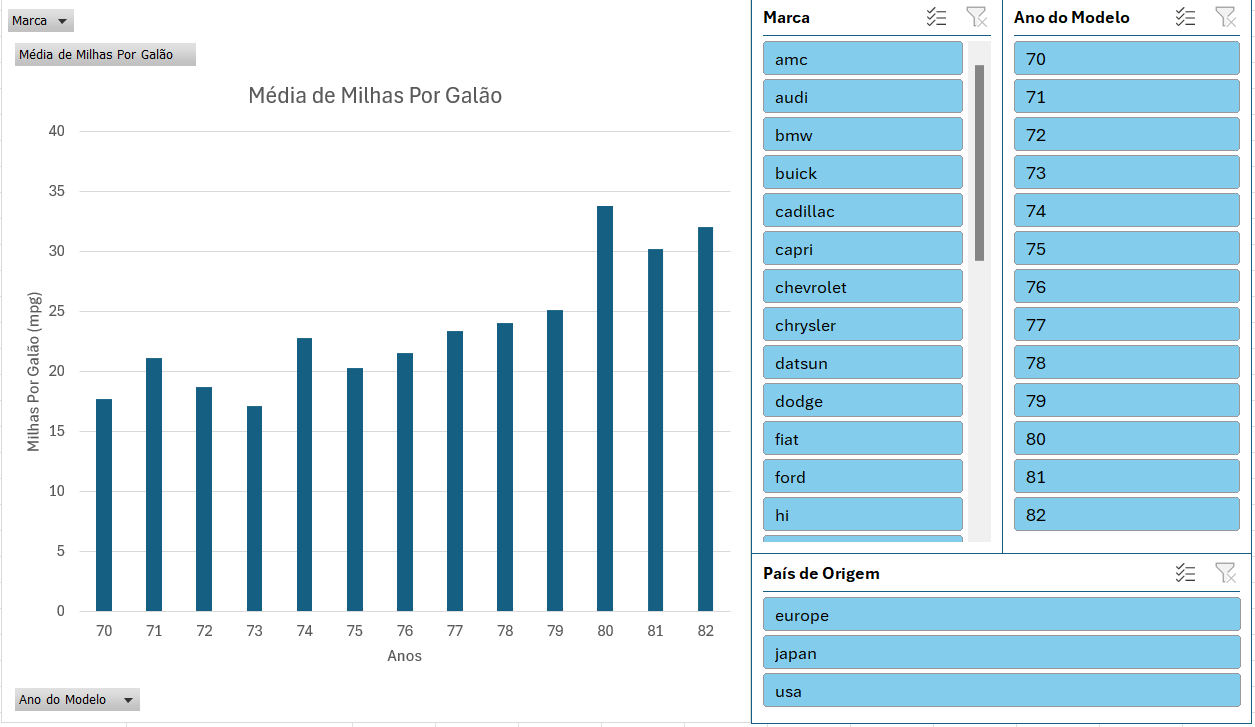
\includegraphics[width=1.2\textwidth]{Recursos/MilhasPorGalaoGrafico.png}
    \vspace{0.5cm}
    \label{fig:mpg}
    \caption{Milhas por galão ao longo dos anos}
\end{figure}
\newpage


%---------------------------------------------------------------------------------------------------------------------------

\subsubsection{Cavalagem}
É possível verificar que a cavalagem dos carros tem diminuido ao longo dos anos, sendo esse um dos motivos
que influenciou a melhoria da eficiência dos carros, pois quanto maior a cavalagem maior o consumo de combustível.
Em 1970 a cavalagem média era de cerca de 150 cavalos e em 1982 a cavalagem média era de cerca de 80 cavalos.
É uma diminuição significativa, que mostra que os carros têm vindo a ser produzidos com motores mais eficientes em termos
de eficiência de combustível, porém sacrificando a sua velocidade e aceleração.

\begin{figure}[h!]
    \centering
    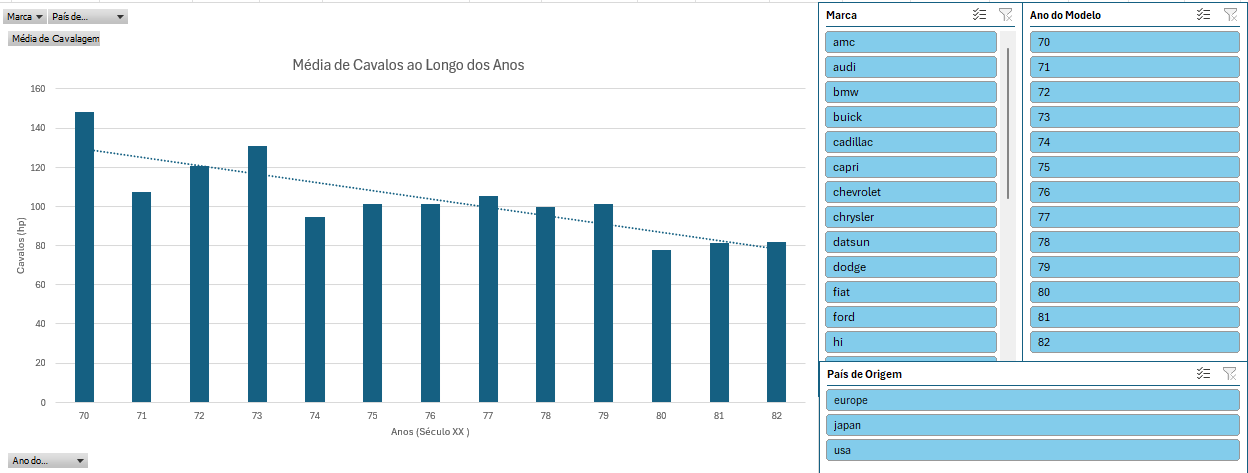
\includegraphics[width=1\textwidth]{Recursos/CavalagemGrafico.png} % Substitua pelo caminho da imagem
    \vspace{0.5cm}
    \label{fig:cavg}
    \caption{Cavalagem ao longo dos anos}
\end{figure}

\newpage
%---------------------------------------------------------------------------------------------------------------------------
\subsubsection{Aceleração Média}
É possível verificar que com a diminuição da cavalagem, o tempo de aceleração dos 0 às 60 milhas por hora dos carros tem vindo a 
aumentar ao longo dos anos, sendo que em 1970 o tempo médio era de cerca de 13 segundos e em 1982 o tempo médio
era de cerca de 16 segundos.
\begin{figure}[h!]
    \centering
    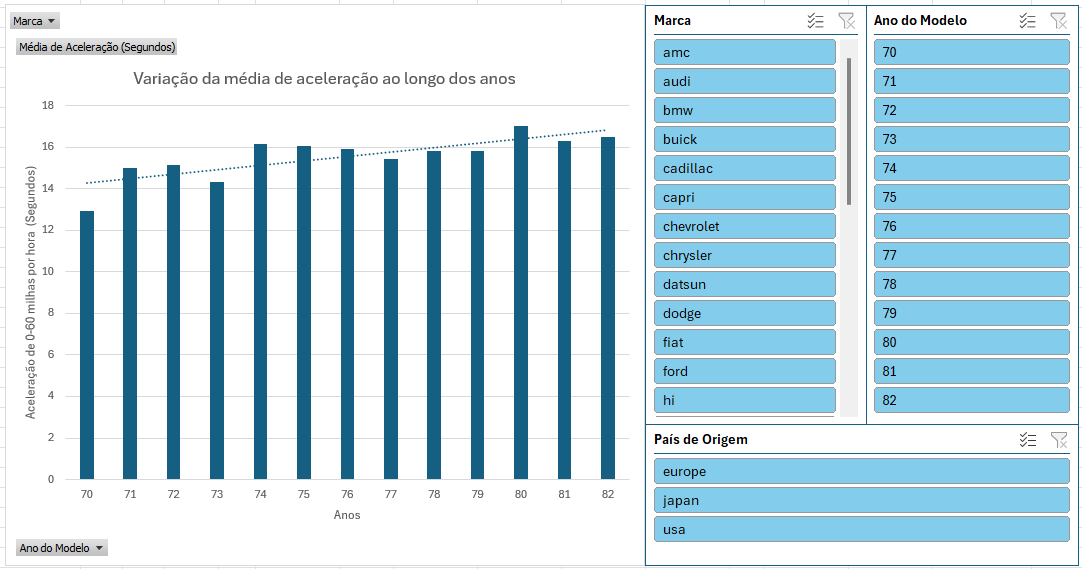
\includegraphics[width=1\textwidth]{Recursos/AceleraçãoMediaGrafico.png} % Substitua pelo caminho da imagem
    \vspace{0.5cm}
    \label{fig:accmg}
    \caption{Aceleração ao longo dos anos}
\end{figure}
\newpage
%---------------------------------------------------------------------------------------------------------------------------
\subsubsection{Número de Veículos}
No gráfico é possível verificar que o número de veículos tem estado estável ao longo dos anos, apesar de 
algumas oscilações, mostrando que o setor automóvel conseguiu adaptar-se à crise do petróleo e manter a produção
de veículos estável. Algumas marcas aumentaram a sua produção, enquanto outras diminuiram.
No entanto, algumas marcas surgiram e outras desapareceram, mostrando que o setor automóvel é muito dinâmico e
está sempre a mudar.

\begin{figure}[h!]
    \centering
    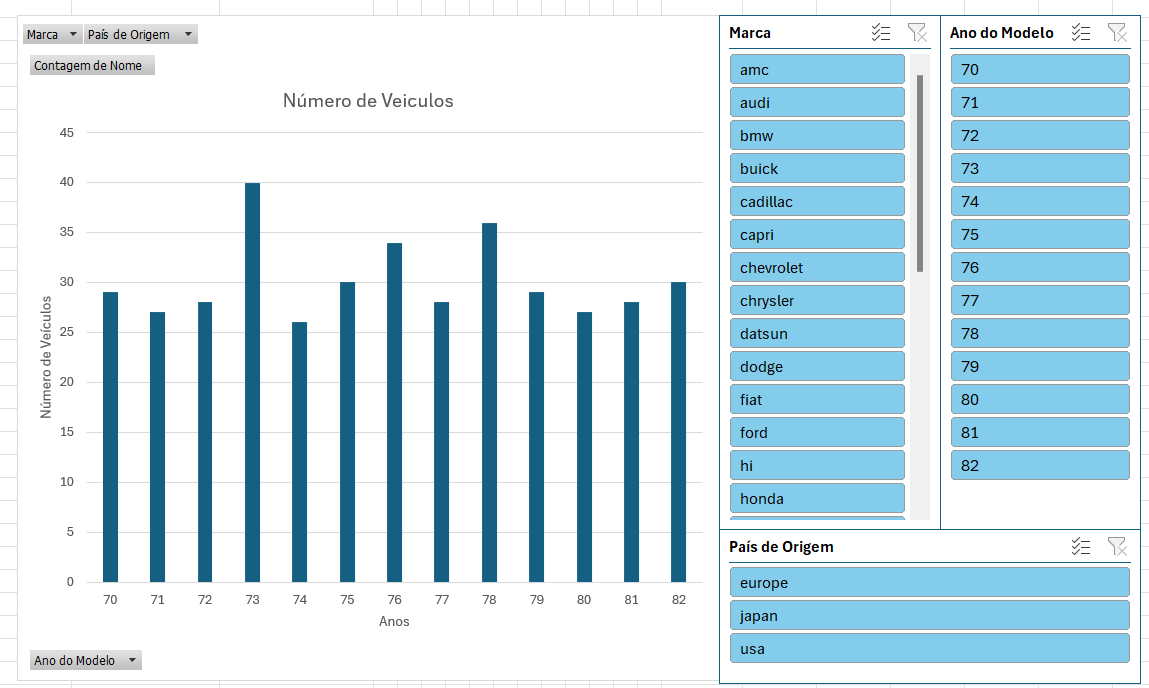
\includegraphics[width=1\textwidth]{Recursos/NVeiculosGrafico.png} % Substitua pelo caminho da imagem
    \vspace{0.5cm}
    \label{fig:nveig}
    \caption{Número de veículos ao longo dos anos}
\end{figure}
\newpage
%---------------------------------------------------------------------------------------------------------------------------
\section{Criação da Data Warehouse}\label{dwh}
\subsection{Metodologia}
O layout da nossa Data Warehouse segue um modelo em estrela ou floco de neve, onde a Tabela de Fato centraliza os dados principais que serão analisados 
(neste caso, métricas como eficiência em combustível, potência, aceleração, etc.) e as Tabelas de Dimensão contêm os atributos contextuais que descrevem as 
características e permitem a segmentação (ex.: ano de fabricação, país de origem). Este layout é vantajoso pois facilita o desempenho das consultas ao 
isolar as medidas principais na tabela fato e os atributos descritivos em tabelas de dimensão, também flexibiliza as análises temporais e comparativas 
ao permitir juntar rapidamente informações, com por exemplo, a eficiência dos carros de diferentes anos e origens.

A Tabela de Fato inclui medidas numéricas (ex.: MPG, cavalagem, aceleração) que podem ser quantificadas e agregadas para gerar insights como médias anuais 
e tendências de eficiência. Isso justifica o agrupamento de métricas centrais (como MPG e cavalagem) na tabela fato, pois são o foco das análises e comparações, 
minimizando a redundância, evitando-se a repetição de dados de contexto (ex.: país ou ano) em todas as entradas, economizando armazenamento e simplificando a estrutura.

As Tabelas de Dimensão, como Ano, País de Origem, e Preço da Gasolina, foram estruturadas para facilitar a segmentação dos dados. A razão para isso inclui a
eficácia em segmentar e filtrar os dados, assim pode-se observar, por exemplo, a produção automóvel de diferentes países face o aumento dos preços de combustível, e o
relacionamento entre tabelas, pois cada Tabela de Dimensão é ligada à Tabela de Fato por uma chave (ex.: ano e país), o que permite consultas rápidas e eficazes.

O layout do diagrama, estruturado para destacar as relações entre atributos de fato e de dimensão, foi feito de forma a facilitar a leitura das relações e dependências 
entre as tabelas, e oferecer flexibilidade para ajustes futuros dado que a organização em um modelo de estrela permite expandir facilmente a Data Warehouse, 
seja adicionando novas métricas (novas colunas na Tabela de Fato) ou novas dimensões (novas Tabelas de Dimensão).

\newpage
\subsection{Diagrama da Data Warehouse}
Assim sendo, esta é a nossa proposta de uma Data Warehouse, dada a nossa análise dos dados.

\begin{figure}[h!]
    \centering
    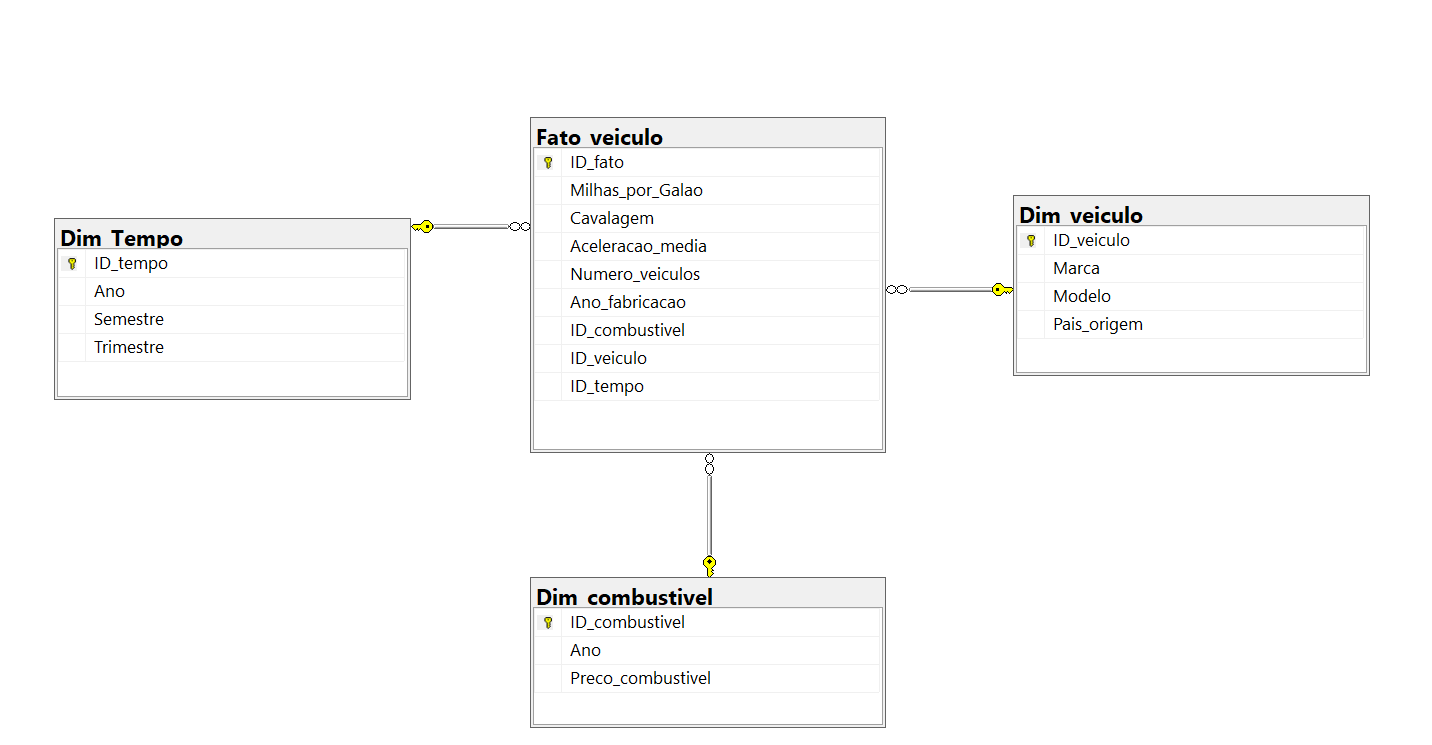
\includegraphics[width=1\textwidth]{Recursos/DiagramaCrisePetroleo.png} % Substitua pelo caminho da imagem
    \vspace{0.5cm}
    \label{fig:dcri}
    \caption{Diagrama da Data Warehouse}
\end{figure}
\newpage
%---------------------------------------------------------------------------------------------------------------------------
\section{Operações OLAP para Análise de Dados}\label{olap}
Foram realizadas operações OLAP, que é a capacidade para manipular e analisar grandes quantidades de dados sob diferentes perspetivas (\cite{moodle}), 
sendo que foram utilizadas as operações de Drill-Down, Roll-Up, Slice e Dice:
\begin{itemize}
    \item \textbf{Drill-Down}: Foi utilizado, por exemplo, para analisar a eficiência em milhas por galão dos carros ao longo dos anos,
    mas ainda assim podendo analisar a eficiência dos carros por país de origem e por marca.
    \item \textbf{Roll-Up}: Esta operação é a inversa da anterior, onde é utilizada ao estar a analisar a eficiência dos carros por país 
    de origem e por marca, o utilizador pode depois analisar a eficiência dos carros ao longo dos anos, independentemente do país de origem e da marca.    
    \item \textbf{Slice}: É utilizado quando é desejado analisar apenas uma fatia da informação, por exemplo, analisar apenas entre 1970 e 1975.
    \item \textbf{Dice}: É utilizado quando o utilizador quer, por exemplo, verificar quais marcas americanas produziram carros entre 1971 e 1979 e 
    verificar a eficiência dos mesmos, seja em aceleração, cavalagem ou autonomia de milhas por galão. 
\end{itemize}
\newpage
%---------------------------------------------------------------------------------------------------------------------------
\section{Contexto Global}\label{cg}

A Crise Petrolífera de 1973 (\cite{pet73}) teve início em outubro de 1973 quando os membros da 
Organização dos Países Árabes Exportadores de Petróleo (OPAEP), que compreende os membros árabes da 
Organização dos Países Exportadores de Petróleo (OPEP), além do Egito e Síria, proclamaram um embargo petrolífero. 
O embargo foi direcionado as nações que eram vistas como apoiantes de Israel durante a Guerra do Yom Kippur. 
As nações alvo do embargo foram inicialmente o Canadá, o Japão, a Holanda, o Reino Unido e os Estados Unidos, 
com o embargo também mais tarde a expandir-se para Portugal, Rodésia e África do Sul. Até o fim do embargo, em março de 1974, 
o preço do petróleo subiu de 3 dólares por barril para cerca de 12 dólares no mundo inteiro. Os preços nos EUA foram ainda mais altos. 
O embargo causou uma crise, ou "choque" de petróleo, com muitos efeitos, de curto ou longo prazo, na política e economia global. 
Mais tarde, foi chamada o "primeiro choque do petróleo", seguido pela crise do petróleo de 1979, chamada o "segundo choque do petróleo."

A Crise Petrolífera de 1979 (\cite{pet79}) ocorreu no mundo devido à diminuição da produção de petróleo após a Revolução Iraniana. 
Apesar das reservas globais de petróleo terem diminuido pouco, o pânico generalizado resultou em uma elevação brusca do preço, 
que aumentou para 39,50 dólares por barril nos 12 meses seguintes, o que formou longas filas em postos de gasolina, como na crise petrolífera de 1973.
%---------------------------------------------------------------------------------------------------------------------------
\section{Conclusão}\label{con}
Estas Crises Petrolíferas fizeram com que os fabricantes de automóveis tivessem de se adaptar e produzir carros mais eficientes, estas adaptações para 
veiculos americanos foram dificeis, cujos quais eram conhecidos por serem grandes e terem motores grandes que gastam muito combustível,
tiveram a sua potencia drasticamente diminuida ao ponto dos modelos desportivos serem considerados muito lentos para a sua categoria.
Os japoneses aproveitaram a situação pois já produziam carros mais pequenos e eficientes e decidiram começar a vender mais no mercado americano,
aumentando a sua quota de mercado significativamente.
%---------------------------------------------------------------------------------------------------------------------------

\newpage
\renewcommand{\refname}{Bibliografia} % Para artigos
\renewcommand{\bibname}{Bibliografia} % Para livros e relatórios
\addcontentsline{toc}{section}{Bibliografia} % Adiciona a Bibliografia ao índice
\printbibliography

\end{document}
